\chapter{Non-linear Classification at the Top}

\section{Introduction}

These problems can be generally written as pushing the positive samples above some decision threshold. The methods differ in the definition of the decision threshold. In our previous work~\cite{adam2021general}, we introduced a general framework that unifies these methods. We showed that several problem classes, which were considered as separate problems so far, fit into the framework. The deficiency of methods from this framework is that they usually cover only linear classifiers. However, as many problems are not linearly separable, nonlinear classifiers are needed. In this work, we show how to extend our framework into nonlinear classification problems. To do so, we use the fact that our framework is similar to the primal formulation of support vector machines~\cite{cortes1995support}. The classical way to incorporate nonlinearity into SVM is to derive the dual formulation~\cite{boyd2004convex} and to employ the kernels method~\cite{scholkopf2001learning}. In this work, we follow this approach, derive dual formulations for the considered problems and add nonlinear kernels to them. Moreover, as dual problems are generally expensive to solve, we derive a quick method to solve them. This is a modification of the coordinate-wise dual ascent from~\cite{hsieh2008dual}. For a review of other approaches see~\cite{batmaz2019review,werner2019review}.

The paper is organized as follows: In Section~\ref{sec:Derivation of dual problems} we recall the unified framework derived in~\cite{adam2021general} and two class of problems that falls into it. Moreover, for selected methods, we derive their dual formulations. Namely, we focus on \TopPush, \TopPushK and \PatMat. In Section~\ref{sec:New method for solving dual problems}, we show how to add nonlinear kernels into dual formulations, derive a new method for solving these dual problems and perform its complexity analysis. Since our method depends on the chosen problem and surrogate function, we provide a concrete form of the solution for \TopPushK with the truncated quadratic loss. Solutions for other problems are provided in Appendix~\ref{sec:Computing Delta with truncated quadratic surrogate} and~\ref{sec:Computing Delta with hinge surrogate}. Finally, in Section~\ref{sec:Numerical experiments} we present the description of performance criteria, choice of hyperparameters and description of datasets. The rest of the section is focused on the results of numerical experiments. Here we compare all methods in terms of overall accuracy and accuracy at a given threshold. We also discuss the convergence and time consumption of all methods. All our codes are available online.\footnote{\texttt{https://github.com/VaclavMacha/ClassificationOnTop\_nonlinear.jl}}

\section{Derivation of dual problems}\label{sec:Derivation of dual problems}

Linear binary classification is a problem of finding a linear hyperplane that separates a group of positive samples from a group of negative samples and achieves the lowest possible error. For a sample~$\bm{x} \in \R^d,$ the prediction for a linear classifier amounts to
\begin{equation*}
  \bm{x} \textnormal{ has }
  \begin{dcases*}
    \textnormal{positive label} & if~$\bm{w}^{\top} \bm{x} \geq t$, \\
    \textnormal{negative label} & otherwise.
  \end{dcases*}
\end{equation*}
Here,~$\bm{w} \in \R^{d}$ is the normal vector to the separating hyperplane and~$t \in \R$ is a decision threshold. The well-known example of such a classifier is a support vector machine~\cite{cortes1995support} where the decision threshold~$t$ is a free variable. However, many important binary classification problems maximize the performance only for a certain amount of samples with the highest scores~$s = \bm{w}^{\top}\bm{x}.$ In these cases, the threshold~$t$ is not a free variable but a function of the scores. In our previous work~\cite{adam2021general}, we formulated a general framework for maximizing performance above the threshold~$t$ as
\begin{equation}\label{eq:General problem}
  \begin{aligned}
    \minimize{\bm{w}, t}
    & \frac{1}{2} \norm{\bm{w}}_{2}^{2} + C \sum_{i = 1}^{n^+} [t - \bm{w}^{\top}\bm{x}^+_{i}] \\
    \st
    & \textnormal{threshold} \ t \ \textnormal{is a function of } \{\bm{w}^{\top} \bm{x_i}\}_{i=1}^n,
  \end{aligned}
\end{equation}
where~$C \in \R$ is a constant;~$[\cdot]$ is the~$0-1$~loss defined as~$1$ if the argument is true and~$0$ otherwise. To denote positive and negative samples, we use~$+$ and~$-$ symbols in the superscript, respectively. Note that~$[t - \bm{w}^{\top}\bm{x}^+_{i}]$ counts the number of positive samples~$\bm x_i^+$ whose score~$\bm{w}^\top \bm x_i^+$ is below the threshold~$t$. Since the objective is to be minimized, the positive samples should lie above the threshold~$t$.

Since the objective function in~\eqref{eq:General problem} is discontinuous due to the~$0-1$~loss, the optimization problem~\eqref{eq:General problem} is difficult. A typical approach to remove this unwanted feature is to approximate the~$0-1$~loss by a surrogate function such as the truncated quadratic or the hinge functions
\begin{align}
    l_{\textnormal{quadratic}}(s)
    & = (\max\{0,1 + \vartheta s\})^{2}, \label{eq:Truncated quadratic loss} \\
    l_{\textnormal{hinge}}(s)
    & = \max\{0,1 + \vartheta s\} \label{eq:Hinge loss},
\end{align}
where~$\vartheta > 0$ is a scaling parameter. In the following text, we use the symbol~$l$ to denote any convex non-negative non-decreasing function with~$l(0) = 1.$ Replacing the~$0-1$~loss in~\eqref{eq:General problem} by a surrogate function results in
\begin{equation}\label{eq:General surrogate problem}
  \begin{aligned}
    \minimize{\bm{w}, t}
    & \frac{1}{2} \norm{\bm{w}}_{2}^{2} + C \sum_{i = 1}^{n^+} l(t - \bm{w}^{\top}\bm{x}^+_{i}) \\
    \st
    & \textnormal{threshold} \ t \ \textnormal{is a function of } \{\bm{w}^{\top} \bm{x_i}\}_{i=1}^n.
  \end{aligned}
\end{equation}
Note that the objective function in~\eqref{eq:General surrogate problem} is continuous.

As we derived in~\cite{adam2021general}, there are many problems belonging to the general framework~\eqref{eq:General problem}. However, this framework handles only linear classification problems. As many problems are not linearly separable, this is often not sufficient. To generalize the framework to nonlinear classifiers, we realize that~\eqref{eq:General surrogate problem} is similar to the primal formulation of the SVM~\cite{cortes1995support}. We will follow the standard way to incorporate nonlinearity into SVM by deriving the dual problem~\cite{boyd2004convex} and using the kernels methods~\cite{scholkopf2001learning}.

In the remainder of this section, we recall two problem classes from~\cite{adam2021general} and their convex approximations, and for each of them, we derive its dual formulation. Namely, we will discuss \TopPushK and \AccatTop with its convex approximation \PatMat.

\subsection{\TopPushK}

The first problem \TopPushK is our modification of the \TopPush method introduced in~\cite{li2014top}. It selects the threshold~$t$ as the mean of the scores corresponding to~$K$ highest ranked negatives. By doing so, it enforces the positives to be ranked above negatives. Therefore, both \TopPush ($K=1$) and \TopPushK ($K>1$) fall into the category of ranking problems.

Writing this more formally, define vector~$\bm{s}$ of all scores as~$s_i = \bm{w}^{\top} \bm{x}_i$ for all~$i = 1, 2, \ldots, n$ and its sorted version~$\bm{s}_{[\cdot]}$ with decreasing components, i.e.~$s_{[1]} \geq s_{[2]} \geq \cdots  \geq s_{[n]}$. Then \TopPushK reads
\begin{equation}\label{eq:TopPushK primal}
  \begin{aligned}
    \minimize{\bm{w}, t, \bm s^-}
    & \frac{1}{2} \norm{\bm{w}}_{2}^{2} + C \sum_{i = 1}^{n^+} l(t - \bm{w}^{\top}\bm{x}^+_{i}) \\
    \st
    & t = \frac{1}{K}\sum_{j = 1}^{K} s^{-}_{[j]}, \\
    & s_j^- = \bm{w}^\top \bm x_j^-, \quad \forall j = 1, 2, \ldots, n^-.
  \end{aligned}
\end{equation}
It can be showed that this problem is convex and that for~$K = 1$ we get the original \TopPush.

In the following theorem, we denote the positive semidefinite kernel matrix~$\K$ by
\begin{equation}\label{eq:kernel_linear}
  \K = \Matrix{\X^+ \\ - \X^-} \Matrix{\X^+ \\ - \X^-}^\top = \Matrix{\X^+ \X^{+\top} & -\X^+ \X^{-\top} \\ -\X^- \X^{+\top} & \X^- \X^{-\top} }.
\end{equation}
and show the form of the \TopPushK dual problem\footnote{To keep the readability of the paper, we postpone all proofs to the Appendix}.

\begin{restatable}[\TopPushK dual formulation]{theorem}{toppushkdual}\label{thm:TopPushK dual}
  The dual problem corresponding to the problem~\eqref{eq:TopPushK primal} has the form
  \begin{subequations}\label{eq:TopPushK dual}
    \begin{alignat}{2}
      \maximize{\bm{\alpha}, \bm{\beta}}
      & - \frac{1}{2} \Matrix{\bm{\alpha} \\ \bm{\beta}}^\top \K \Matrix{\bm{\alpha} \\ \bm{\beta}} - C \sum_{i = 1}^{n^+} l^{\star}\Brac{\frac{\alpha_i}{C}} \span \span \label{eq:TopPushK dual objective} \\
      \st
      & \sum_{i = 1}^{n^+} \alpha_i = \sum_{j = 1}^{n^-} \beta_j, \label{eq:TopPushK dual constraint 1} \\
      & 0 \leq \beta_j \leq \frac{1}{K} \sum_{i = 1}^{n^+} \alpha_i,  && \quad \forall j = 1, 2, \ldots, n^-, \label{eq:TopPushK dual constraint 2}
    \end{alignat}
    where~$l^{\star}$ is a conjugate of the surrogate loss function~$l$ from~\eqref{eq:TopPushK primal} and~$\K$ was defined in~\eqref{eq:kernel_linear}.
  \end{subequations}
\end{restatable}

\subsection{\AccatTop}

The second problem \AccatTop was introduced in~\cite{boyd2012accuracy}. On the contrary to \TopPushK, which focuses on the minimization of the number of positive samples below~$K$~highest ranked negatives, the \AccatTop minimizes the number of positive samples below the top~$\tau$-quantile from negative samples defined as
\begin{equation}\label{eq:Quantile}
    t = \max \Set{t}{\sum_{j = 1}^{n^-} [\bm{w}^\top \bm{x}_j^- - t] \geq n \tau}.
\end{equation}
Then \AccatTop is an optimization problem written as follows
\begin{equation}\label{eq:AccAtTop}
  \begin{aligned}
    \minimize{\bm{w}, t}
    & \frac{1}{2} \norm{\bm{w}}_{2}^{2} + C \sum_{i = 1}^{n^+} l_1(t - \bm{w}^{\top}\bm{x}^+_{i}) \\
    \st
    & t \ \textnormal{is the surrogate top} \ \tau\textnormal{-quantile: it solves~\eqref{eq:Quantile}}.
  \end{aligned}
\end{equation}
Since it is known that the quantile function~\eqref{eq:Quantile} is non-convex, we derived its convex surrogate approximation
\begin{equation}\label{eq:Surrogate quantile}
  t \quad \textnormal{solves} \quad \sum_{j = 1}^{n^-} l_2(\bm{w}^{\top}\bm{x}_{j}^- - t) \leq n \tau.
\end{equation}
Replacing the true quantile~\eqref{eq:Quantile} by its surrogate approximation~\eqref{eq:Surrogate quantile} yields
\begin{equation}\label{eq:PatMat primal}
  \begin{aligned}
    \minimize{\bm{w}, t}
    & \frac{1}{2} \norm{\bm{w}}_{2}^{2} + C \sum_{i = 1}^{n^+} l_1(t - \bm{w}^{\top}\bm{x}^+_{i}) \\
    \st & t \ \textnormal{is the top} \ \tau\textnormal{-quantile: it solves~\eqref{eq:Surrogate quantile}}.
  \end{aligned}
\end{equation}
In~\cite{adam2021general}, we called the convex problem~\eqref{eq:PatMat primal} \PatMat. The following theorem shows its dual form.

\begin{restatable}[\PatMat dual formulation]{theorem}{patmatdual}\label{thm:PatMat dual}
  The dual problem corresponding to the problem~\eqref{eq:PatMat primal} has the form
  \begin{subequations}\label{eq:PatMat dual}
    \begin{align}
      \maximize{\bm{\alpha}, \bm{\beta}, \delta}
      & -\frac{1}{2} \Matrix{\bm{\alpha} \\ \bm{\beta}}^\top \K \Matrix{\bm{\alpha} \\ \bm{\beta}} - C \sum_{i = 1}^{n^+} l_1^{\star} \Brac{\frac{\alpha_i}{C}} - \delta \sum_{j = 1}^{n^-} l_2^{\star} \Brac{\frac{\beta_j}{\delta}} - \delta n \tau \label{eq:PatMat dual objective} \\
      \st
      & \sum_{i = 1}^{n^+} \alpha_i = \sum_{j = 1}^{n^-} \beta_j, \label{eq:PatMat dual constraint 1} \\
      & \delta \geq 0, \label{eq:PatMat dual constraint 2} 
    \end{align}
    where~$l_1^{\star}$,~$l_2^{\star}$ are conjugates of the surrogate loss functions~$l_1,$~$l_2$ from~\eqref{eq:PatMat primal} and~$\K$ was defined in~\eqref{eq:kernel_linear}.
  \end{subequations}
\end{restatable}

\section{New method for solving dual problems}\label{sec:New method for solving dual problems}

In the previous section, we derived the dual formulations for the \TopPushK and \PatMat problems. These dual formulations allow us to incorporate nonlinearity using kernels~\cite{scholkopf2001learning} in the same way as in SVM. Since the dimension of~\eqref{eq:TopPushK dual} and~\eqref{eq:PatMat dual} equals to the number of samples~$n$, it is computationally expensive to use standard techniques such as the gradient descent. To handle this issue, the coordinate descent algorithm~\cite{chang2008coordinate,hsieh2008dual} has been proposed in the context of SVMs. Since problems~(\ref{eq:TopPushK dual},~\ref{eq:PatMat dual}) differ from original SVMs by additional constraints (\ref{eq:TopPushK dual constraint 1},~\ref{eq:PatMat dual constraint 1}), the key idea of our algorithm is to update two coordinates (instead of one) of~$\bm{\alpha},$~$\bm{\beta}$ at every iteration. To summarize, we will solve the original tasks~(\ref{eq:TopPushK dual},~\ref{eq:PatMat dual}) by an iterative procedure where in every iteration we need to find a solution of a one-dimensional quadratic optimization problem. As we will show later, these one-dimensional problems have a closed form solution, which means that every iteration is cheap.

\subsection{Adding kernels}

To add kernels, we realize first that from the proofs of Theorems~\ref{thm:TopPushK dual} and~\ref{thm:PatMat dual} for any~$\bm{z}\in\R^d$ we have
\begin{equation}\label{eq:pred_linear}
  \bm{w}^\top \bm{z} = \sum_{i = 1}^{n^+} \alpha_i \bm{z}^\top \bm{x}^+_i - \sum_{j = 1}^{n^-} \beta_j \bm{z}^\top \bm{x}^-_j
\end{equation}
Consider now any kernel function~$k:\R^d\times\R^d\to\R$. Using the standard trick, we replace the kernel matrix~\eqref{eq:kernel_linear} by\footnote{
The first part of the objective of~\eqref{eq:TopPushK dual} and~\eqref{eq:PatMat dual} amounts to
\begin{equation*}
  \Matrix{\bm{\alpha} \\ \bm{\beta}}^\top \K \Matrix{\bm{\alpha} \\ \bm{\beta}}
  = \Matrix{\bm{\alpha} \\ \bm{\beta}}^\top \Matrix{\X^+ \X^{+\top} & -\X^+ \X^{-\top} \\ -\X^- \X^{+\top} & \X^- \X^{-\top} }\Matrix{\bm{\alpha} \\ \bm{\beta}}
  = \Matrix{\bm{\alpha} \\ -\bm{\beta}}^\top \Matrix{\X^+ \X^{+\top} & \X^+ \X^{-\top} \\ \X^- \X^{+\top} & \X^- \X^{-\top} }\Matrix{\bm{\alpha} \\ -\bm{\beta}},
\end{equation*}
from which~\eqref{eq:kernel_nonlinear} follows.}
\begin{equation}\label{eq:kernel_nonlinear}
  \K = \Matrix{k(\X^+, \X^{+}) & -k(\X^+, \X^{-}) \\ -k(\X^-, \X^{+}) & k(\X^-, \X^{-}) },
\end{equation}
where~$k(\cdot,\cdot)$ is applied to all rows of both arguments. Then for a new sample~$\bm{z}$, the prediction~\eqref{eq:pred_linear} is replaced by
\begin{equation}\label{eq:pred_nonlinear}
  \textrm{pred}(\bm{z}) = \sum_{i = 1}^{n^+} \alpha_i k\left(\bm{z}, \bm{x}^+_i\right) - \sum_{j = 1}^{n^-} \beta_j k\left(\bm{z}, \bm{x}^-_j\right),
\end{equation}
where~$\bm{\alpha}$ and~$\bm{\beta}$ are the optimal solution of~\eqref{eq:TopPushK dual} or~\eqref{eq:PatMat dual}.

\subsection{Update of dual optimization variables}

Let us consider the kernel matrix~$\K$ as in~\eqref{eq:kernel_nonlinear} and define the score vector~$\bm{s}$ by
\begin{equation}\label{eq:defin_s}
    \bm{s} = \K \Matrix{\bm{\alpha} \\ \bm{\beta}}.
\end{equation}
There are three possible update rules which modify two coordinates of~$\bm{\alpha},$~$\bm{\beta}$ and which satisfy constraints (\ref{eq:TopPushK dual constraint 1},~\ref{eq:PatMat dual constraint 1}) and keep~\eqref{eq:defin_s} satisfied. The first one updates two components of~$\bm{\alpha}$
\begin{subequations}\label{eq:Update rules}
  \begin{equation}\label{eq:Update rule a,a}
    \begin{alignedat}{2}
      \alpha_k & \rightarrow \alpha_k + \Delta, & \qquad
      \alpha_l & \rightarrow \alpha_l - \Delta, & \qquad
      \bm{s}   & \rightarrow \bm{s} + (\K_{\bullet k} - \K_{\bullet l})\Delta,
    \end{alignedat}
  \end{equation}
  where~$K_{\bullet i}$ denotes~$i$-th column of~$\K.$ Note that the update rule for~$\bm{s}$ does not use matrix multiplication but only vector addition. The second rule updates one component of~$\bm{\alpha}$ and one component of~$\bm{\beta}$ 
  \begin{equation}\label{eq:Update rule a,b}
    \begin{alignedat}{2}
      \alpha_k & \rightarrow \alpha_k + \Delta, & \qquad
      \beta_l  & \rightarrow \beta_l  + \Delta, & \qquad
      \bm{s}   & \rightarrow \bm{s} + (\K_{\bullet k} + \K_{\bullet l})\Delta,
    \end{alignedat}
  \end{equation}
  and the last one updates two components of~$\bm{\beta}$
  \begin{equation}\label{eq:Update rule b,b}
    \begin{alignedat}{2}
      \beta_k & \rightarrow \beta_k + \Delta, & \qquad
      \beta_l & \rightarrow \beta_l - \Delta, & \qquad
      \bm{s}  & \rightarrow \bm{s} + (\K_{\bullet k} - \K_{\bullet l})\Delta.
    \end{alignedat}
  \end{equation}
\end{subequations}
These three update rules hold true for any surrogate function. However, the calculation of the optimal~$\Delta$ depends on the used problem formulation and surrogate function. In Subsection~\ref{sec:Computing Delta for TopPushK with truncated quadratic loss}, we show the closed-form formula for~$\Delta$ for \TopPushK problem~\eqref{eq:TopPushK dual} with truncated quadratic surrogate function~\eqref{eq:Truncated quadratic loss}. Computation of~$\Delta$ for the hinge surrogate or \PatMat is presented in Appendices~\ref{sec:Computing Delta with truncated quadratic surrogate} and~\ref{sec:Computing Delta with hinge surrogate}. 

\subsection{Algorithm summary and Complexity analysis}

We summarize the whole procedure in Algorithm~\ref{alg:Coordinate descent}. We will describe it only for \PatMat (right column) as for \TopPushK (left column) it is almost identical. In step~\ref{alg: line 1} we initialize~$\bm{\alpha}$,~$\bm{\beta}$ and~$\delta$ to some feasible value and based on~\eqref{eq:defin_s} compute~$\bm s$. Each \repeatloop loop in step~\ref{alg: line 2} updates two coordinates as shown in~\eqref{eq:Update rules}. In step~\ref{alg: line 3} we select a random index~$k$ and in the \forloop loop in step~\ref{alg: line 4} we compute the optimal~$(\Delta_l,\delta_l)$ for all possible combinations~$(k,l)$ as in~\eqref{eq:Update rules}. In step~\ref{alg: line 7} we select the pair~$(\Delta_l,\delta_l)$ which maximizes the objective. Finally, based on~\eqref{eq:Update rules} we update~$\bm{\alpha}$,~$\bm{\beta}$,~$\bm s$ and~$\delta$ in steps~\ref{alg: line 8} and~\ref{alg: line 9}.

\begin{algorithm*}[!ht]
  \begin{minipage}{0.48\textwidth}
    \centering
    \begin{algorithmic}[1]
      \State set~$(\bm{\alpha}, \bm{\beta})$ feasible, set~$\bm{s}$ based on \eqref{eq:defin_s} \label{alg: line 1}
      \Repeat \label{alg: line 2}
        \State select random~$k$ from~$\{1, 2, \ldots, n\}$ \label{alg: line 3}
        \For{$l \in \{1, 2, \ldots, n\}$} \label{alg: line 4}
            \State compute~$\Delta_{l}$  \label{alg: line 5}
        \EndFor
        \State select best~$\Delta_{l}$ \label{alg: line 7}
        \State update~$\bm{\alpha}$,~$\bm{\beta},$~$\bm{s}$ according to~\eqref{eq:Update rules} \label{alg: line 8}
        \State \label{alg: line 9}
      \Until{stopping criterion is satisfied}
    \end{algorithmic}
  \end{minipage}
  \hfill
  \begin{minipage}{0.51\textwidth}
    \centering
    \begin{algorithmic}[1]
      \State set~$(\bm{\alpha}, \bm{\beta}, \delta)$ feasible, set~$\bm{s}$ based on \eqref{eq:defin_s}
      \Repeat
        \State select random~$k$ from~$\{1, 2, \ldots, n\}$ 
        \For{$l \in \{1, 2, \ldots, n\}$}
            \State compute~$(\Delta_{l}, \; \delta_{l})$
        \EndFor
        \State select best~$(\Delta_{l}, \; \delta_{l})$
        \State update~$\bm{\alpha}$,~$\bm{\beta},$~$\bm{s}$ according to~\eqref{eq:Update rules}
        \State set~$\delta \leftarrow \delta_{l}$
      \Until{stopping criterion is satisfied}
    \end{algorithmic}
  \end{minipage}
  \caption{Coordinate descent algorithm for \TopPushK (left) and \PatMat (right).}
  \label{alg:Coordinate descent}
\end{algorithm*}

Now we derive the computational complexity of each \repeatloop loop from step~\ref{alg: line 2}. Since the computation of~$(\Delta_l,\delta_l)$ amounts to solving a quadratic optimization problem in one variable, there is a closed-form solution (see Section~\ref{sec:Computing Delta for TopPushK with truncated quadratic loss}) and step~\ref{alg: line 5} can be performed in~$O(1)$. Since this is embedded in a \forloop loop in step~\ref{alg: line 4}, the whole complexity of this loop is~$O(n)$. Step~\ref{alg: line 8} requires~$O(1)$ for the update of~$\bm{\alpha}$ and~$\bm{\beta}$ while~$O(n)$ for the update of~$\bm s$. Since the other steps are~$O(1)$, the total complexity of the \repeatloop loop is~$O(n)$. This holds true only if the kernel matrix~$\K$ is precomputed. In the opposite case, all complexities must by multiplied by the cost of computation of components of~$\K$ which is~$O(d)$. This complexity analysis is summarized in Table~\ref{tab:Computational complexity}. 


\begin{table}[!ht]
  \centering
  \begin{tabular}{@{}clll@{}l} 
    \toprule
    Precomputed~$\K$ & Evaluation of~$\Delta_l$ & Update of~$\bm{s}$ & Total per iteration \\
    \midrule
    \yesmark & $O(1)$ & $O(n)$  & $O(n)$ \\
    \nomark  & $O(d)$ & $O(nd)$ & $O(nd)$ \\
    \bottomrule
  \end{tabular}
  \caption{Computational complexity of one \repeatloop loop (which updates two coordinates of~$\bm{\alpha}$ or~$\bm{\beta}$) from Algorithm~\ref{alg:Coordinate descent}.}
  \label{tab:Computational complexity}
\end{table}

\subsection{Computing~$\Delta$ for \TopPushK with truncated quadratic loss}\label{sec:Computing Delta for TopPushK with truncated quadratic loss}

In this section, we show how to compute the stepsize~$\Delta$ from~\eqref{eq:Update rules} for \TopPushK~\eqref{eq:TopPushK dual} with the truncated quadratic surrogate function~\eqref{eq:Truncated quadratic loss}. Optimal~$\Delta$ for \PatMat can be found in a similar way as we show in Appendix~\ref{sec:Computing Delta with truncated quadratic surrogate}. In Appendix~\ref{sec:Computing Delta with hinge surrogate} we present the computation of optimal~$\Delta$ for \TopPushK and \PatMat with the hinge loss function~\eqref{eq:Hinge loss}.

Plugging the conjugate~\eqref{eq:Conjugate of truncated quadratic loss} of the truncated quadratic loss~\eqref{eq:Truncated quadratic loss} into \TopPushK dual formulation~\eqref{eq:TopPushK dual} yields
\begin{subequations}\label{eq:TopPushK dual quadratic}
  \begin{alignat}{2}
    \maximize{\bm{\alpha}, \bm{\beta}}
    & - \frac{1}{2} \Matrix{\bm{\alpha} \\ \bm{\beta}}^\top \K \Matrix{\bm{\alpha} \\ \bm{\beta}} + \frac{1}{\vartheta} \sum_{i = 1}^{n^+} \alpha_i - \frac{1}{4 C \vartheta^2} \sum_{i = 1}^{n^+} \alpha_i^2 \span \span \label{eq:TopPushK dual quadratic objective} \\
    \st 
    & \sum_{i = 1}^{n^+} \alpha_i = \sum_{j = 1}^{n^-} \beta_j, \label{eq:TopPushK dual quadratic constraint 1} \\
    & \alpha_i \geq 0, && \quad \forall i = 1, 2, \ldots, n^+, \label{eq:TopPushK dual quadratic constraint 2} \\
    & 0 \leq \beta_j  \leq \frac{1}{K} \sum_{i = 1}^{n^+} \alpha_i, && \quad \forall j = 1, 2, \ldots, n^-. \label{eq:TopPushK dual quadratic constraint 3}
  \end{alignat}
\end{subequations}
This is a quadratic optimization problem. Moreover, for~$K=1$ the upper bound in~\eqref{eq:TopPushK dual quadratic constraint 3} automatically follows from~\eqref{eq:TopPushK dual quadratic constraint 1} and the problem can be simplified. In the following theorem, we show that for each of update rules~\eqref{eq:Update rules}, problem~\eqref{eq:TopPushK dual quadratic} has a simple closed-form solution. For simplicity, we use~$\clip{a}{b}{c}$ to denote clipping (projecting)~$c$ to the interval~$[a,b]$.

\begin{restatable}[Update rule for~$\Delta^*$ for \TopPushK with truncated quadratic loss]{theorem}{toppushkupdatequadratic}\label{thm:Update rule TopPushK with quadratic loss}
  Consider problem~\eqref{eq:TopPushK dual quadratic}. Then the optimal step~$\Delta^\star$ equals to
  \begin{equation}\label{eq:Optimal delta}
    \Delta^{*} = \clip{\Delta_{lb}}{\Delta_{ub}}{\gamma},
  \end{equation}
  where there are the following three cases (each corresponding to one update rule in~\eqref{eq:Update rules}):
  \begin{itemize}
    \item For any~$1\le k, l \le n^+$ we have
    \begin{align*}
      \Delta_{lb} & = -\alpha_k, \\
      \Delta_{ub} & = \alpha_l, \\
      \gamma      & = -\frac{s_k - s_l + \frac{1}{2C\vartheta^2}(\alpha_k - \alpha_l)}{\K_{kk} + \K_{ll} - \K_{kl} - \K_{lk} + \frac{1}{C\vartheta^2}}.
    \end{align*}
    \item For any~$1 \le k \le n^+$ and~$n^+ + 1 \le l \le n$ we define~$\hat{l} = l - n^+$  and~$\beta_{\max} = \max_{j \in \{1, 2, \ldots, n^- \} \setminus \{\hat l\}} \beta_j.$ Then we have
    \begin{align*}
      \Delta_{lb} & = 
        \begin{cases*}
          \max \Brac[c]{- \alpha_k,\;  -\beta_{\hat l}} & K = 1, \\
          \max \Brac[c]{- \alpha_k,\;  -\beta_{\hat l}, \; K\beta_{\max} - \sum_{i = 1}^{n^+} \alpha_i} & \textrm{otherwise},
        \end{cases*} \\
      \Delta_{ub} & = 
        \begin{cases*}
          + \infty & K = 1, \\
          \frac{1}{K-1}\Brac{\sum_{i = 1}^{n^+} \alpha_i - K \beta_{\hat l}} & \textrm{otherwise},
        \end{cases*} \\
      \gamma & = -\frac{s_k + s_l - \frac{1}{\vartheta} + \frac{1}{2C\vartheta^2} \alpha_k}{\K_{kk} + \K_{ll} + \K_{kl} + \K_{lk} + \frac{1}{2C\vartheta^2}}.
    \end{align*}
    \item For any~$n^+ + 1\le k,l \le n$ we define~$\hat{k} = k - n^+,$~$\hat{l} = l - n^+$ and then  have
    \begin{align*}
      \Delta_{lb} & = 
        \begin{cases*}
          -\beta_{\hat k} & K = 1, \\
          \max \Brac[c]{- \beta_{\hat k},\; \beta_{\hat l} - \frac{1}{K} \sum_{i = 1}^{n^+} \alpha_i} & \textrm{otherwise},
        \end{cases*} \\
      \Delta_{ub} & = 
        \begin{cases*}
          \beta_{\hat l} & K = 1, \\
          \min \Brac[c]{\beta_{\hat l},\; \frac{1}{K} \sum_{i = 1}^{n^+} \alpha_i - \beta_{\hat k}} & \textrm{otherwise},
        \end{cases*} \\
      \gamma & = -\frac{s_k - s_l}{\K_{kk} + \K_{ll} - \K_{kl} - \K_{lk}}.
    \end{align*}
  \end{itemize}
\end{restatable}

\section{Numerical experiments}\label{sec:Numerical experiments}

In this section, we present numerical results. All codes were implemented in the Julia language~\cite{bezanson2017julia} and are available online.\footnote{All codes are available at \url{https://github.com/VaclavMacha/ClassificationOnTop_new.jl}}

\subsection{Performance criteria}

For the evaluation of numerical experiments, we use precision and recall. For a threshold~$t$ they are defined by
\begin{equation}\label{eq:prec_rec}
  \begin{alignedat}{2}
      \precision
      & = \frac{\sum_{i = 1}^{n^+} [\bm{w}^{\top}\bm{x}^+_{i} - t]}{\sum_{i = 1}^{n} [\bm{w}^{\top}\bm{x}_{i} - t]}, & \qquad
      \recall
      & = \frac{1}{n^+} \sum_{i = 1}^{n^+} [\bm{w}^{\top}\bm{x}^+_{i} - t].
  \end{alignedat}
\end{equation}
We also use the Precision-Recall (PR) curve that are commonly used for unbalanced data~\cite{davis2006relationship} and precision at a certain level of recall which we denote by~$\pratrec$.

\subsection{Hyperparameter choice}

In Section~\ref{sec:New method for solving dual problems} we introduced Algorithm~\ref{alg:Coordinate descent} for solving dual problems~(\ref{eq:TopPushK dual},~\ref{eq:PatMat dual}). We let it run for~$20000$ \repeatloop loops, which corresponds to~$40000$ updates of coordinates of~$(\bm{\alpha},\bm{\beta})$. We use the linear and Gaussian kernels defined by
\begin{align}
  k_{\textrm{lin}}(\bm{x}, \bm{y})   & = \bm{x}^{\top} \bm{y}, \label{eq:Linear kernel} \\
  k_{\textrm{gauss}}(\bm{x}, \bm{y}) & = \exp\{-\sigma \norm{\bm{x} - \bm{y}}_2^2\} \label{eq:Gaussian kernel}
\end{align}
and the truncated quadratic loss~\eqref{eq:Truncated quadratic loss} with~$\vartheta = 1$ as a surrogate. 

The classifiers were trained on the training set. We selected the optimal hyperparameter from
\begin{equation*}
  \begin{aligned}
    \tau   & \in \{0.01,\ 0.05,\ 0.1\}, &
    K      & \in \{5,\ 10\}, &
    C      & \in \{0.1,\ 1,\ 10\}, &
    \sigma & \in \{0.01,\ 0.05\} 
  \end{aligned}
\end{equation*}
which gave the best performance on the validation set. All presented result are shown on the testing set which was not part of the training process.

\begin{table}[ht]
  \centering
  \begin{tabular}{@{}lllllllll@{}}
      \toprule
      &&& \multicolumn{2}{c}{Training}
        & \multicolumn{2}{c}{Validation}
        & \multicolumn{2}{c}{Testing} \\
      \cmidrule(lr){4-5} \cmidrule(lr){6-7} \cmidrule(l){8-9}
        & $y^+$
        & $d$
        & $n$
        & $\frac{n^+}{n}$
        & $n$
        & $\frac{n^+}{n}$
        & $n$
        & $\frac{n^+}{n}$ \\
      \midrule
      sigillito1989classification
        & -- & 34 & 176 & 64.2\% & 87 & 64.4\% & 88 & 63.6\% \\
      Spambase
        & -- & 57 & 2301 & 39.4\% & 1150 & 39.4\% & 1150 & 39.4\% \\
      WhiteWineQuality
        & 7, 8, 9 & 11 & 2449 & 21.6\% & 1224 & 21.7\% & 1225 & 21.6\% \\
      RedWineQuality
        & 7, 8 & 11 & 800 & 13.5\% & 400 & 13.8\% & 399 & 13.5\% \\
      Fashion-MNIST
        & 0 & 784 & 50000 & 10.0\% & 10000 & 10.0\% & 10000 & 10.0\% \\
      \bottomrule
  \end{tabular}
  \caption{Summary of the used datasets. It shows which original labels~$y^+$ were selected as the positive class, the number of features~$d,$ samples~$n,$ and the fraction of positive samples~$\frac{n^+}{n}$.}
  \label{tab:Datasets}
\end{table}

\subsection{Dataset description}

For numerical experiments, we consider the FashionMNIST dataset~\cite{xiao2017fashionmnist} and four smaller datasets from the UCI repository~\cite{dua2019uci}: sigillito1989classification~\cite{sigillito1989classification}, Spambase, WhiteWineQuality~\cite{cortez2009modeling} and RedWineQuality~\cite{cortez2009modeling}. Datasets that do not contain testing set were randomly divided into a training (50\%), validation (25\%) and testing (25\%) sets. For datasets that contain a testing set, the training set was randomly divided into a training and a validation set, where the validation set has the same size as the testing set. FashionMNIST dataset was converted to binary classification tasks by selecting class with label 0 as the positive class and the rest as the negative class. All datasets are summarized in Table~\ref{tab:Datasets}.

\subsection{Experiments}

In Figure~\ref{fig:PR comparison} we present the PR curves for all methods with two different kernels evaluated on the FashionMNIST dataset. The left column corresponds to the linear kernel~\eqref{eq:Linear kernel} while the right one to the Gaussian kernel~\eqref{eq:Gaussian kernel} with~$\sigma = 0.01$. The nonlinear Gaussian kernel significantly outperforms the linear kernel. This will be confirmed later in Table~\ref{tab:Metrics comparison} where we present a comparison from multiple datasets. 

\begin{figure}[!ht]
  \centering
  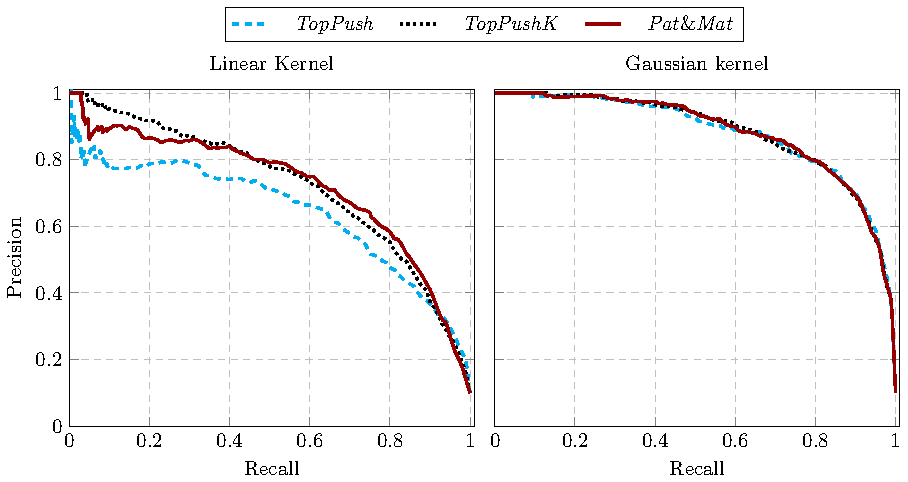
\includegraphics[width = \linewidth]{images/dual_results1.pdf}
  \caption{PR curves for all methods and  FashionMNIST dataset. The left column corresponds to the linear kernel~\eqref{eq:Linear kernel} and the right column corresponds to the Gaussian kernel~\eqref{eq:Gaussian kernel}.}
  \label{fig:PR comparison}
\end{figure}

For a better illustration of how the methods from Figure~\ref{fig:PR comparison} work, we present density estimates of scores~$\bm s$ from \eqref{eq:defin_s}. High scores predict positive labels while low scores predict negative labels. The rows of Figure~\ref{fig:Scores comparison} depict the linear \eqref{eq:Linear kernel} and the Gaussian kernels \eqref{eq:Gaussian kernel} with~$\sigma = 0.01$ while each column corresponds to one method. The black vertical lines depict the top 5\%-quantile of all scores (on the testing set). Since a smaller overlap of scores of samples with positive and negative labels implies a better separation, we deduce the benefit of the Gaussian over the linear kernel.

\begin{figure}[!ht]
  \centering
  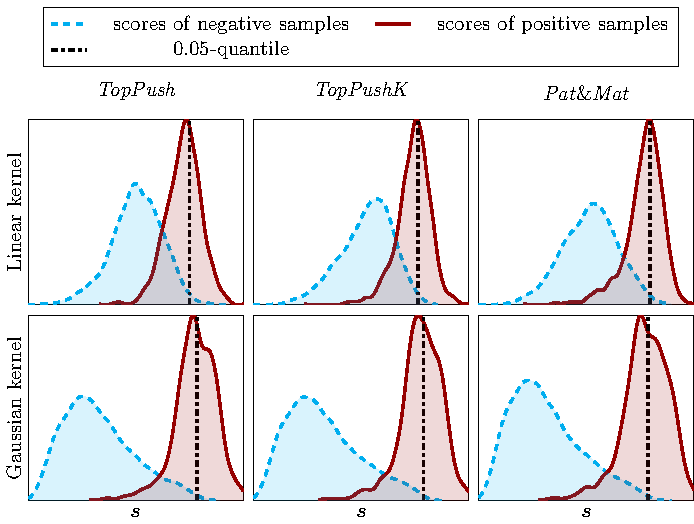
\includegraphics[width = \linewidth]{images/dual_results2.pdf}
  \caption{Density estimates for scores corresponding to samples with positive and negative labels for the FashionMNIST dataset.}
  \label{fig:Scores comparison}
\end{figure}

In Table~\ref{tab:Metrics comparison} we present the precision of all methods across all datasets from Table~\ref{tab:Datasets}. For each dataset, we trained each method and computed precision at certain levels of recall. The depicted values are averages over all datasets. For each kernel and each level of recall, the best precision is highlighted in light green. Moreover, the best overall precision for each level of recall is depicted in dark green. We can make several observations from Table~\ref{tab:Metrics comparison}:
\begin{itemize}
  \item All methods perform better with the Gaussian kernels than with the linear kernel. 
  \item \TopPush and \TopPushK perform better for sufficiently small recall. This happened because they consider the threshold to be the maximal~$K$ negative scores and small recall corresponds to high threshold. However, for the same reason, \TopPush is not robust.
  \item \PatMat is the best for all kernels if the recall is sufficiently large. The reason is again the form of the decision threshold.
\end{itemize}

\begin{table}[ht]
  \centering
  \begin{tabular}{@{}c|llllllll@{}}
    \toprule
    \multicolumn{3}{c}{} & \multicolumn{6}{c}{$\pratrec$}  \\
    \cmidrule(lr){4-9}
    \multicolumn{3}{c}{}
      & 0.05 & 0.1 & 0.2 & 0.4 & 0.6 & 0.8 \\
    \midrule
    \multirow{6}{*}{\rotatecell{Linear kernel}}
    & \TopPush
      & & \best 79.83 & 64.27 & \best 65.55 & 61.85 & 57.89 & 51.83 \\
    & \TopPushK & $K = 5$
      & 73.96 & \best 65.41 & 64.82 & 60.28 & 56.94 & 50.52 \\
    & & $K = 10$
      & 60.63 & 61.97 & 59.69 & 56.89 & 54.40 & 49.83 \\
    & \PatMat & $\tau = 0.01$
      & 63.67 & 60.30 & 58.74 & 57.75 & 53.32 & 48.42 \\
    & & $\tau = 0.05$
      & 54.05 & 60.91 & 63.32 & 55.24 & 52.55 & 48.30 \\
    & & $\tau = 0.1$
      & 57.02 & 61.24 & 62.49 & \best 63.11 & \best 59.91 & \best 52.14 \\
    \midrule
    \multirow{6}{*}{\rotatecell{Gaussian kernel}}
    & \TopPush
      & & \besttotal 97.50 & 86.06 & 81.28 & 76.15 & 71.13 & 60.17 \\
    & \TopPushK & $K = 5$
      & 92.50 & 87.56 & 85.31 & 78.47 & 70.77 & 57.10 \\
    & & $K = 10$
      & 89.50 & 87.56 & 83.15 & 79.09 & 71.88 & 59.27 \\
    & \PatMat & $\tau = 0.01$
      & 89.65 & \besttotal 89.11 & \besttotal 86.75 & 80.77 & 75.44 & 65.95 \\
    & & $\tau = 0.05$
      & 80.77 & 81.28 & 85.74 & 82.92 & 74.91 & 65.04 \\
    & & $\tau = 0.1$
      & 81.30 & 84.14 & 82.58 & \besttotal 83.12 & \besttotal 77.82 & \besttotal 66.50 \\
    \bottomrule
  \end{tabular}
  \caption{The precision of all methods averaged across all datasets from Table~\ref{tab:Datasets}. Each column represents precision at a certain level of recall. Light green depicts the best method for the given kernel and dark green depicts the best overall method.}
  \label{tab:Metrics comparison}
\end{table}

In Figure~\ref{fig:Convergence comparison}, we investigate the convergence of methods. In each column, we show the convergence of primal and dual problems for one method. To solve the primal problem, we use the gradient method proposed in~\cite{adam2021general}. For the dual problem, we use our Algorithm~\ref{alg:Coordinate descent}. Since~\cite{adam2021general} considers only linear kernels, we present them. Moreover, since the computation of the objective is expensive, the results are presented for the sigillito1989classification dataset. We can see that \TopPush and \TopPushK converge to the same objective for primal and dual problems. This means that the problem was solved to optimality. However, there is a little gap between optimal solution of primal and dual problems for \PatMat.

\begin{figure}[!ht]
  \centering
  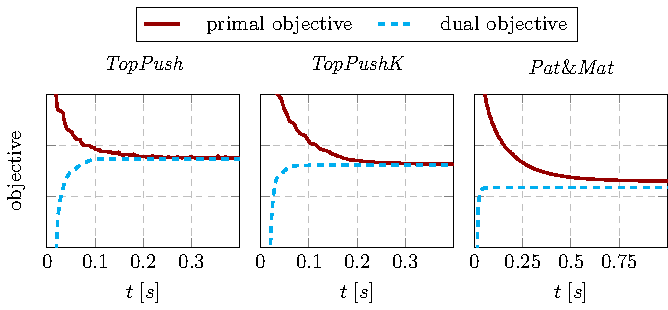
\includegraphics[width = \linewidth]{images/dual_results3.pdf}
  \caption{Convergence of the objectives for the primal (red line) and dual (blue line) problems for the sigillito1989classification dataset with linear kernel.}
  \label{fig:Convergence comparison}
\end{figure}

Finally, Table~\ref{tab:Time comparison} depicts the time comparison for all methods and all datasets. It shows the average time in milliseconds needed for one \repeatloop loop in Algorithm~\ref{alg:Coordinate descent}. The time is relatively stable and for most of the datasets it is below one millisecond. Since we run all experiments for 20000 \repeatloop loops, the evaluation of one method with one hyperparameter setting takes a few seconds for smaller datasets and approximately 7 minutes for FashionMNIST. The average time for one~$\Delta_l$ in step~\ref{alg: line 5} in Algorithm~\ref{alg:Coordinate descent} took between~$1.7\cdot 10^{-7}$ and~$3.1\cdot 10^{-7}$ seconds for each methods. It is almost the same for all datasets, which corresponds to the fact that the complexity of step~\ref{alg: line 5} is independent of the size of the dataset. Note that in all experiments we used precomputed kernel matrix~$\K$ saved on the hard drive and not in memory.

\begin{table}[ht]
  \centering
  \begin{tabular}{@{}c|llll@{}}
      \toprule
      \multicolumn{2}{c}{}
        & \TopPush & \TopPushK & \PatMat \\
      \midrule
      \multirow{5}{*}{\rotatecell{One \repeatloop \\ loop [ms]}}
      & sigillito1989classification
        & $ 0.04 \pm 0.00 $ & $ 0.03 \pm 0.00 $ & $ 0.03 \pm 0.00 $ \\
      & Spambase
        & $ 0.56 \pm 0.02 $ & $ 0.49 \pm 0.01 $ & $ 0.50 \pm 0.01 $ \\
      & WhiteWineQuality
        & $ 0.62 \pm 0.03 $ & $ 0.53 \pm 0.01 $ & $ 0.54 \pm 0.01 $ \\
      & RedWineQuality
        & $ 0.17 \pm 0.01 $ & $ 0.14 \pm 0.01 $ & $ 0.15 \pm 0.01 $ \\
      & Fashion-MNIST
        & $ 17.16 \pm 0.74 $ & $ 15.95 \pm 0.14 $ & $ 15.54 \pm 0.80 $ \\
      \bottomrule
  \end{tabular}
  \caption{The average time with standard deviation (in milliseconds) for one \repeatloop loop in Algorithm~\ref{alg:Coordinate descent}. The average time for one~$\Delta_l$ in step~\ref{alg: line 5} in Algorithm~\ref{alg:Coordinate descent} took between~$1.7\cdot 10^{-7}$ and~$3.1\cdot 10^{-7}$ seconds for each methods.}
  \label{tab:Time comparison}
\end{table}

\section{Conclusion}\label{sec:Conclusion}

In this paper, we analyzed and extended the general framework for binary classification on top samples from~\cite{adam2021general} to nonlinear problems. Achieved results can be summarized as follows:
\begin{itemize}
    \item We derived the dual formulations for \TopPush, \TopPushK and \PatMat.
    \item We proposed a new method for solving the dual problems. We performed its complexity analysis. For selected surrogate functions we also derived the exact formulas needed in the method.
    \item We performed a numerical analysis of the proposed method. We showed its good convergence as well as improved performance of nonlinear kernels over the linear one.
\end{itemize}
Based on the numerical analysis from Section~\ref{sec:Numerical experiments}, we recommend using \TopPush or \TopPushK for problems where the resulting recall should be small. Otherwise, we recommend using \PatMat with an appropriately selected~$\tau$ parameter.
